\chapter{Il Sistema Internazionale e i campioni delle unità di misura}

\begin{figure}[h]
    \centering
    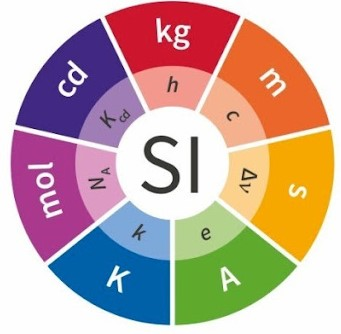
\includegraphics[scale = 1]{Nuovo SI Simbolo.jpg}
\end{figure}

\newpage 

\begin{tcolorbox}
Questo capitolo sarà di tipo nozionistico e culturale: non è necessario un enorme approfondimento tecnico.     
\end{tcolorbox}

\section{Organismi per la metrologia} 
\footnote{Slide della prof | SDME 1.3 Metrologia - SI e Campioni | pag 2 - 6 \\  
Appunti | 2025-02-28 | pag 6}

La metrologia è la scienza delle misure. \newline 

Nel 1875, a Parigi, viene siglata la Convenzione del Metro. \newline 

Ci sono degli organismi internazionali che si occupano della metrologia. \newline 

Dal punto di vista gerarchico, quindi dall'alto verso il basso, avremo: 

\begin{itemize}
    \item CGPM (Conferenza Generale dei Pesi e delle Misure): possiamo considerarlo come l'ente politico che è responsabile delle iniziative per la diffusione del Sistema Internazionale adottato nel 1960 
    \item BIPM (Ufficio Internazionale dei Pesi e delle Misure): è l'ente tecnico del CGPM 
    \item CIPM (Comitato Internazionale dei Pesi e delle Misure): è un organo tecnico-scientifico in cui ci sono insediati i comitati consultativi a cui sono delegati i problemi tecnici  
    \item OIML (Organismo Internazionale per la Metrologia Legale): si occupa del settore della metrologia legale che ha implicazioni negli ambiti economico, della salute e della sicurezza 
    \item NMI (Istituti Metrologici Nazionali): svolgono attività di ricerca, realizzano e conservano i campioni primari delle diverse nazioni 
    In Italia abbiamo:
    \begin{itemize} 
        \item INRiM (Istituto Nazionale di Ricerca Metrologica): si occupa di tutti i diversi settori della metrologia, tranne le radiazioni ionizzanti  
        \item INMRI (Istituto Nazionale di Metrologia delle Radiazioni Ionizzanti)
    \end{itemize}
\end{itemize}

Un importante organismo per la metrologia in Italia è Accredia, che è un ente indipendente, unico nel nostro paese, che gestisce l'accreditamento dei laboratori di taratura, 
o LAT (Laboratori Accreditati di Taratura). \newline 

I LAT, conservano i campioni secondari distribuiti sul territorio nazionale e, periodicamente, vengono confrontati con il campione di riferimento nazionale, per garantire la riferibilità. \newline 

\newpage 

\section{Unità di misura e sistemi di unità di misura} 
\footnote{Slide della prof | SDME 1.3 Metrologia - SI e Campioni | pag 8 \\
Appunti | 2025-06-23 Ricevimento | pag 1 - 2}

Un'unità di misura è un termine di riferimento adottato, per convenzione, per confrontare una grandezza con altre, della stessa specie.\newline 

I campioni delle u.d.m. consentono di rendere tangibili le unità di misura. \newline 

Per campione di u.d.m. tangibile si intende che la realizzazione pratica dell'u.d.m. è una realizzazione facilmente realizzabile: 
è come il campione dell'ampere che, per definirlo, serve un banale circuito di 1 V e un resisotre da 1 $\Omega$ , 
rispetto al campione dell'u.d.m. del tempo in cui non possiamo realizzare la velocità della luce. \newline 

Un particolare insieme di unità di misura che consentono di riferire le misure a campioni 
unitari convenzionalmente riconosciuti, è detto sistema di unità di misura. \newline 

I sistemi di unità di misura possono essere: 
\begin{itemize}
    \item non coerenti, si fornisce una definizione per ciascuna u.d.m 
    \item coerenti, si definiscono solamente le u.d.m. di base e si ricavano le u.d.m. derivate 
\end{itemize}

Le grandezze fisiche a cui si riferiscono le u.d.m. di un sistema sono tra loro indipendenti, 
mentre possono non esserlo le u.d.m. stesse. \newline 

\newpage 

\section{Il sistema internazionale (SI) di unità di misura} 
\footnote{Slide della prof | SDME 1.3 Metrologia - SI e Campioni | pag 9 - 10}

Negli anni sono stati proposti e usati in paesi diversi sistemi di riferimento, fino a oggi che si usa il Sistema Internazionale (SI) di unità di misura, 
cioè il sistema più diffuso e internazionalmente riconosciuto, ufficialmente impiegato in quasi tutti i paesi del mondo (esclusi Liberia, Birmania e USA). \newline 

\begin{tcolorbox}
    Perchè gli americani sono americani e poi sbagliano i calcoli quando vanno su Marte \\
    \url{https://sci4dem.it/un-errore-di-conversione-costoso-il-caso-della-sonda-mars-climate-orbiter/}
\end{tcolorbox}

Il SI si basa su sette u.d.m. fondamentali: 

{
\Large 
\begin{center}
    \begin{tabular}{c  c  c}
        \textbf{Grandezza} & \textbf{u.d.m} & \textbf{Impiego} \\ 
        metro & [m] & per la lunghezza \\
        chilogrammo & [kg] & perla massa \\ 
        secondo & [s] & per l'intervallo di tempo \\
        ampere & [A] & per per la corrente elettrica \\
        kelvin & [K] & per la temperatura \\ 
        mole & [mol] & per la quantità di sostanza \\ 
        candela & [cd] & per l'intensità luminosa
    \end{tabular}        
\end{center}

}

\newpage 

\footnote{Slide della prof | SDME 1.3 Metrologia - SI e Campioni | pag 7}

Per effettuare misure abbiamo bisogno di riferimenti di misura espressi nella stessa unità di misura della grandezza misurata. \newline 

Particolari riferimenti di misura, sono detti unità di misura (o u.d.m). \newline 

Dal punto di vista rappresentativo, possiamo scrivere che la grandezza misurata ha fornito un valore G: 

{
    \Large 
    \begin{equation}
        \text{G = VAL X U}
    \end{equation}
    
}

in cui il valore adimensionale VAL viene applicato all'unità di misura U. \newline 

Essendo VAL un numero reale, G e U devono essere la stessa u.d.m.:  \\

{
    \Large 
    \begin{equation}
        \text{[G] = [U]}
    \end{equation}
    
}


\newpage

\footnote{Slide della prof | SDME 1.3 Metrologia - SI e Campioni | pag 9 - 10}

L'SI dalla sua origine nel 1889 si è evoluto, fino ad arrivare ai giorni d'oggi. \newline 

Nel 1960 si sta cercando di eliminare la dipendenza da esperimenti o manufatti specifici. \newline 

Nel 2018, il 26esimo CGPM ha stabilito il nuovo SI. \newline 

Il nuovo SI ruota intorno alla definizione di 7 costanti di natura, 
dalle quali è possibile ricavare le 7 u.d.m. fondamentali, 
e quindi anche ogni altra unità di misura SI. \newline 

Ci si riferisce all'SI ridefinito nel 2019 come "nuovo SI" (e si usa oggi riferirsi all'SI del 1971 come "vecchio SI"). \newline

\newpage 

\section{"Vecchio" SI (1960-2019)}
\footnote{Slide della prof | SDME 1.3 Metrologia - SI e Campioni | pag 12 - 17 \\  
Appunti | 2025-02-28 | pag 6 - 8}

Di seguito, le definizioni del metro e del chilogrammo: 

\begin{figure}[h]
    \centering
    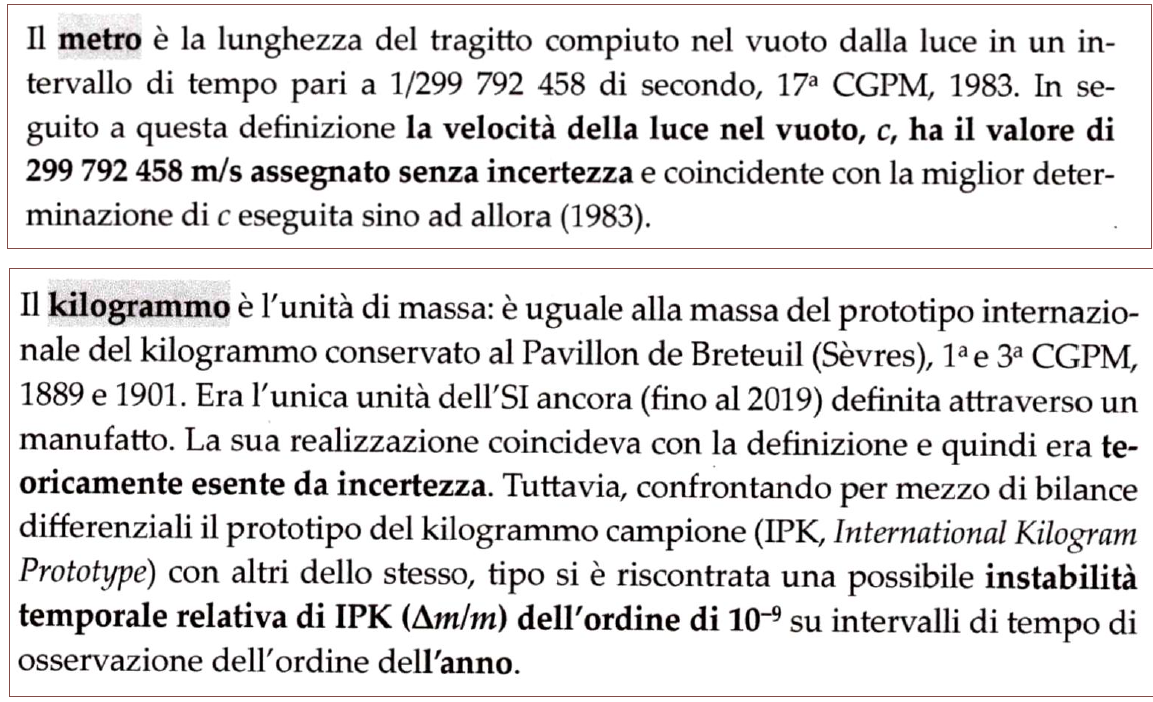
\includegraphics[scale = 0.5]{Definizio del metro e del kilogrammo dal vecchio SI.PNG}
\end{figure}

Tra vecchio e "nuovo" SI non sono state modificate tutte le definizioni delle grandezze fondamentali. \newline 

\begin{figure}[h]
    \centering
    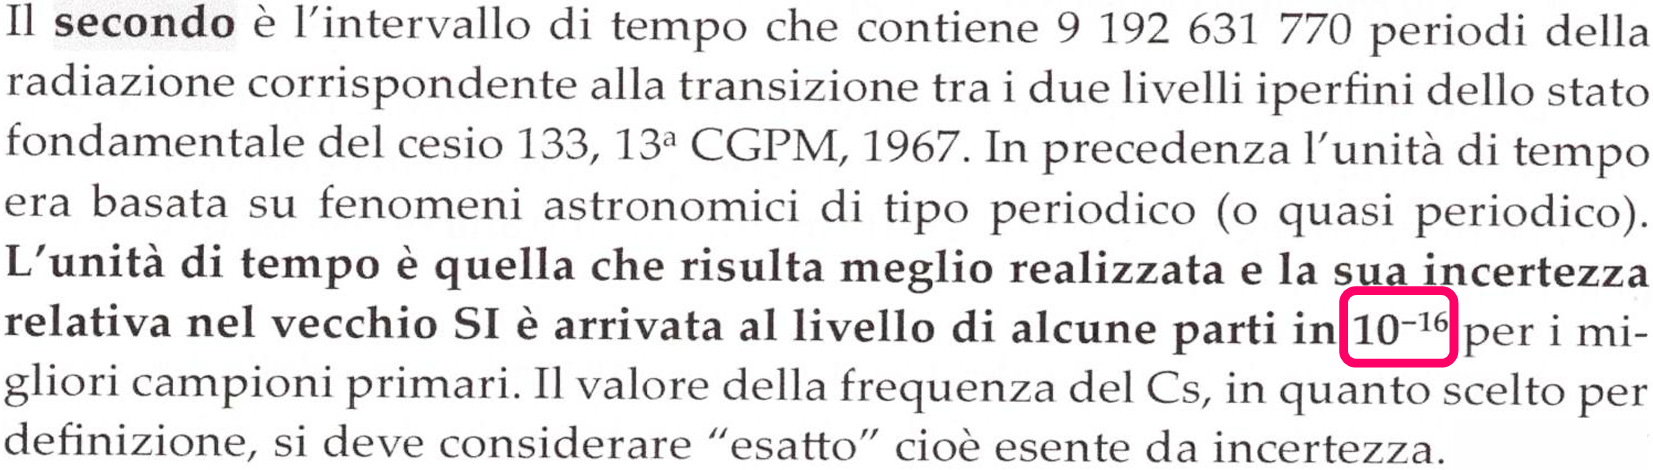
\includegraphics[scale = 0.3]{Definizione del secondo dal vecchio SI.PNG}
\end{figure}

I segnali di tempo sono gli unici che possono essere trasmessi a distanza senza richiedere il trasporto del campione. \newline 

La loro diffusione è essenziale in applicazioni come i segnali orari, la sincronizzazione delle reti di trasmissione dati o dei sistemi di navigazione satellitare. \newline 

Dalla definizione del tempo, notiamo che se un termine è assoluto, gli altri fenomeni sono multipli interi dal campione assoluto. \newline 

Inoltre, essendo il termine assoluto, sarà costante in tutto il mondo e nei diversi esperimenti perché il loro valore cambierà in tanto tempo (generalmente si parla di millenni). \newline 

Considerando l'importanza dei segnali di tempo, si è ritenuto di stabilire una scala di tempo universalmente riconosciuta - UTC (Universal Time Coordinated). \newline 

Ora diamo la definizione dell'ampere: 

\begin{figure}[h]
    \centering
    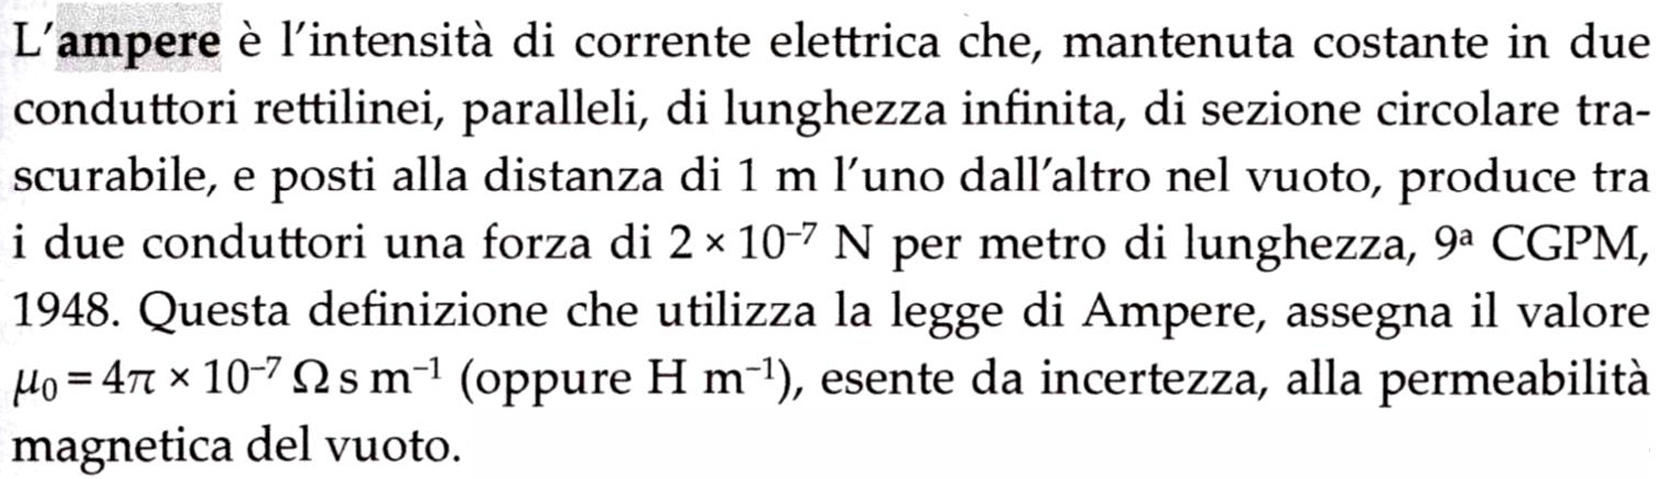
\includegraphics[scale = 0.3]{Definizione dell'ampere dal vecchio SI.PNG}
\end{figure}

\newpage

Sempre dal "Vecchio" SI, di seguito riporto le definizioni di kelvin, mole e candela: 

\begin{figure}[h]
    \centering
    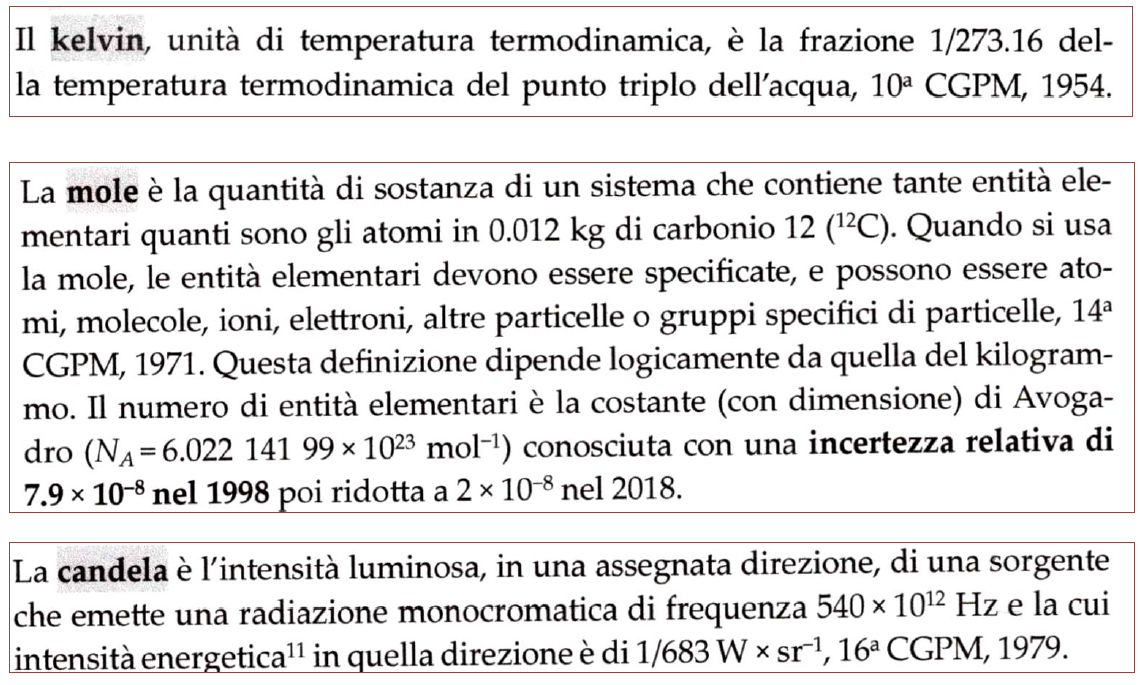
\includegraphics[scale = 0.5]{Definizione del kelvin, mole e candela dal vecchio SI.PNG}
\end{figure}


Con il "Vecchio" SI, è possibile definire la relazione di dipendenza tra le 7 unità di base con il seguente schema: 

\begin{figure}[h]
    \centering
    \includegraphics[scale = 0.2]{Relazione 7 unità di base del vecchio SI.png}
\end{figure}

\newpage 

Le quantità o grandezze fisiche di base dietro ciascuna unità o grandezze fisiche di base 
dietro ciascuna unità dell'SI sono, per convenzione, ritenute indipendenti tra loro. \newline 

Invece le unità di misura dell'SI non risultano tra loro indipendenti. \newline 

\newpage 

\section{Nuovo SI (in vigore dal 2019)}
\footnote{Slide della prof | SDME 1.3 Metrologia - SI e Campioni | pag 18 - 24 \\  
Appunti | 2025-02-28 | pag 8 - 9}

In seguito alla sua profonda revisione, divenuta operativa nel maggio del 2019, 
l'SI rimane basato su 7 u.d.m di base che sono definite attraverso 7 costanti di natura. \newline 

Tutte le nostre misurazioni in ambito SI, sia prima che dopo il 2019, 
sono in ultima analisi riferite ai campioni (dette anche mise en pratique, o realizzazioni pratiche in Italiano ). \newline 

Le definizioni di secondo, metro e candela non sono sostanzialmente cambiate, 
mentre per le altre 4 unità (kilogrammo, ampere, kelvin e mole) le ridefinizioni adottate nel 2019 sono sostanziali. \newline 

Grazie al seguente schema è possibile definire le grandezze fondamentali e le loro costanti fondamentali: 

\begin{figure}[h]
    \centering
    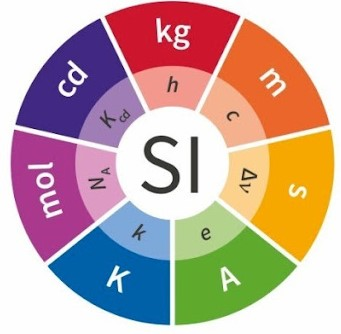
\includegraphics[scale = 0.3]{Nuovo SI Simbolo.jpg}
\end{figure}

Il Sistema Internazionale di unità di misura, SI, è un sistema che si base sulle seguenti 
costanti prive di incertezza, dette anche costanti assolute: 

\begin{itemize}
    \item la frequenza di transizione iperfine del livello fondamentale dell'atomo di cesio 133 è 
    {
        \Large 
        \begin{equation}
            \Delta_{v_{Cs}} = 9\text{ }192 \text{ }631 \text{ } 770 \text{ } Hz
        \end{equation}

    } 

    \item la velocità della luce nel vuoto è: 
    {
        \Large 
        \begin{equation}
            c = 299 \text{ } 792 \text{ } 458 \text{ } m/s
        \end{equation}

    }

    \item la costante di Planck è: 
    {
        \Large 
        \begin{equation}
            h = 6.626\text{}070\text{}15 \times 10^{-34} J \cdot s
        \end{equation}
    }
    
    \item la carica elementare è: 
    {
        \Large 
        \begin{equation}
            e = 1.602\text{}176\text{}634 \times 10^{-19}\text{} C
        \end{equation}
    }
    
    \item la costante di Boltzmann è:
    {
        \Large 
        \begin{equation}
            k = 1.380 \text{}649 \times 10^{-23} \text{} \frac{J}{K}
        \end{equation}
    } 
    
    \item la costante di Avogadro è: 
    {
        \Large 
        \begin{equation}
            N_A = 6.022 \text{} 140 \text{} 76 \times 10^{23} \text{ } mol^{-1}
        \end{equation}
    }
    
    \item la efficienza di una radiazione monocromatica di frequenza $540 \times 10^{12}$ Hz è:  
    {
        \Large
        \begin{equation}
            K_{cd} = 683 \text{ } \frac{lm}{W}
        \end{equation}
    }
\end{itemize}


\begin{tcolorbox}
    Per i nostri studi, 
    le costanti più importanti sono quella della transizione del cesio 133, 
    la velocità della luce nel vuoto e 
    la carica elementare
\end{tcolorbox}

\newpage 

Di seguito le definizioni delle unità di misura del nuovo SI (riporto solo quelle che ci interesseranno nel corso): 

\begin{figure}[h]
    \centering
    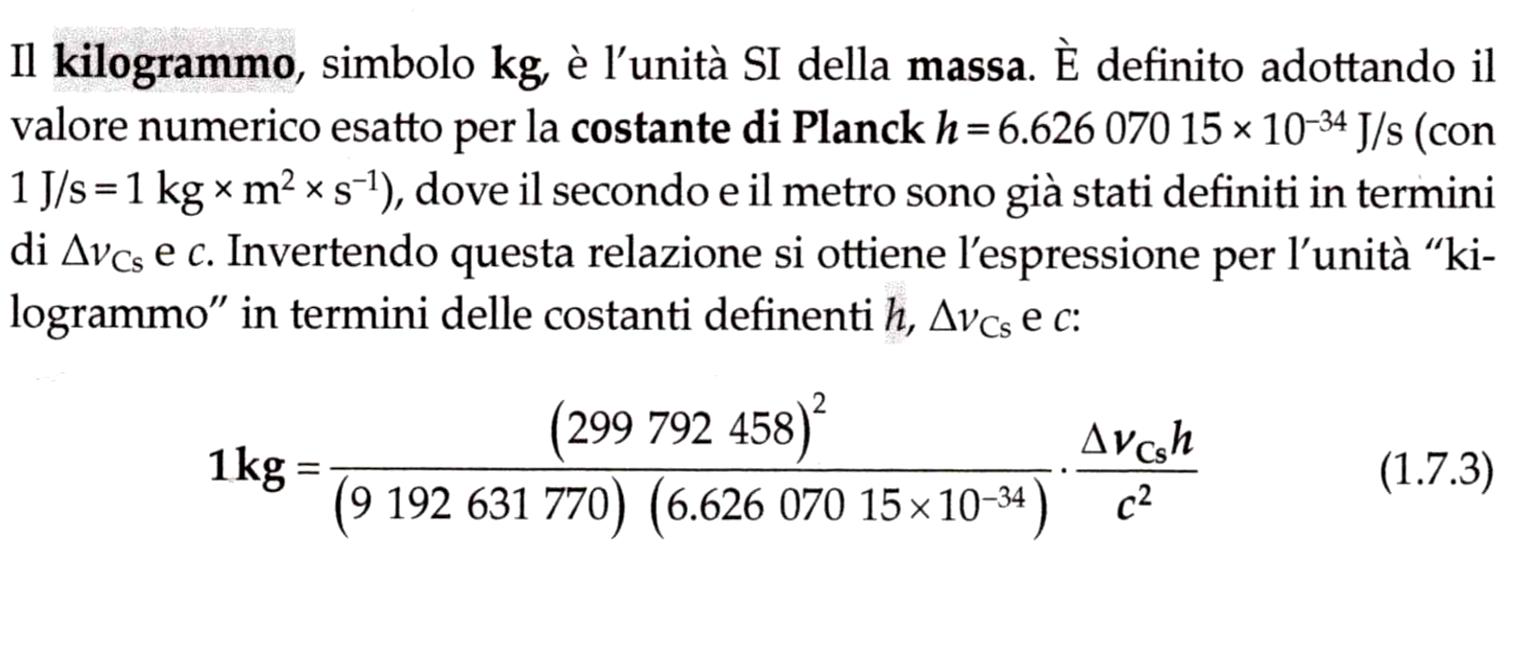
\includegraphics[scale = 0.3]{Definizione del kilogrammo dal nuovo SI.png}
    \\
    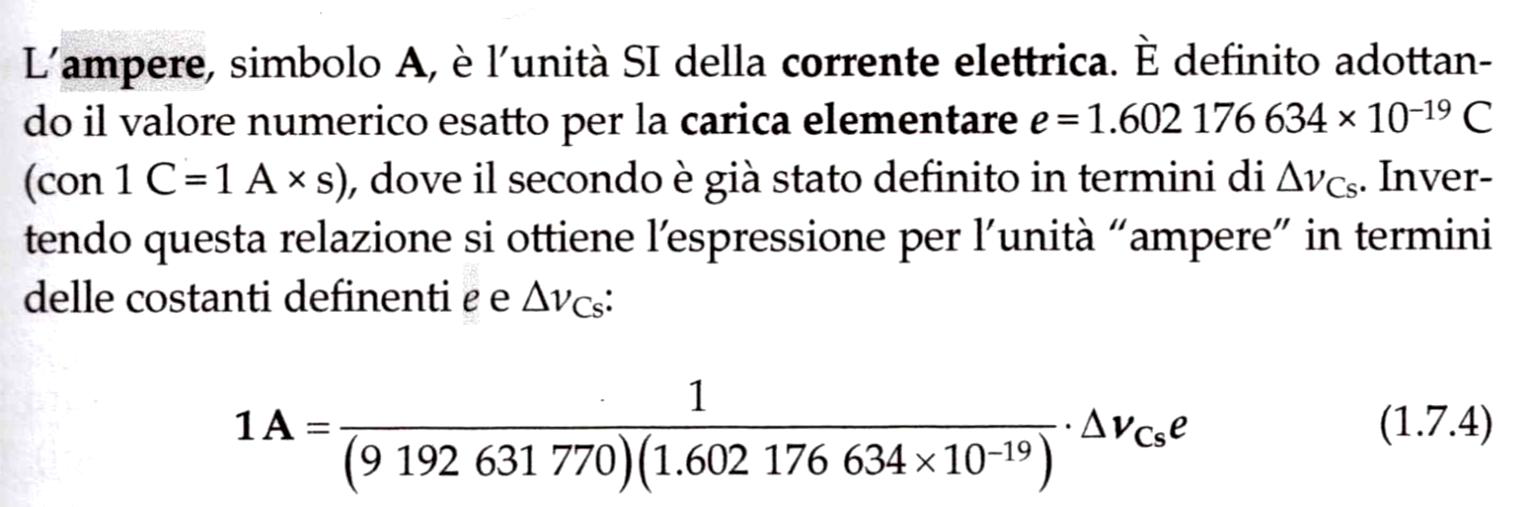
\includegraphics[scale = 0.3]{Definizione dell'ampere dal nuovo SI.png}
\end{figure}

Grazie al seguente schema, 
è possibile confrontare le relazione tra le grandezze del nuovo SI con il vecchio SI ed i loro artefatti: 

\begin{figure}[h]
    \centering
    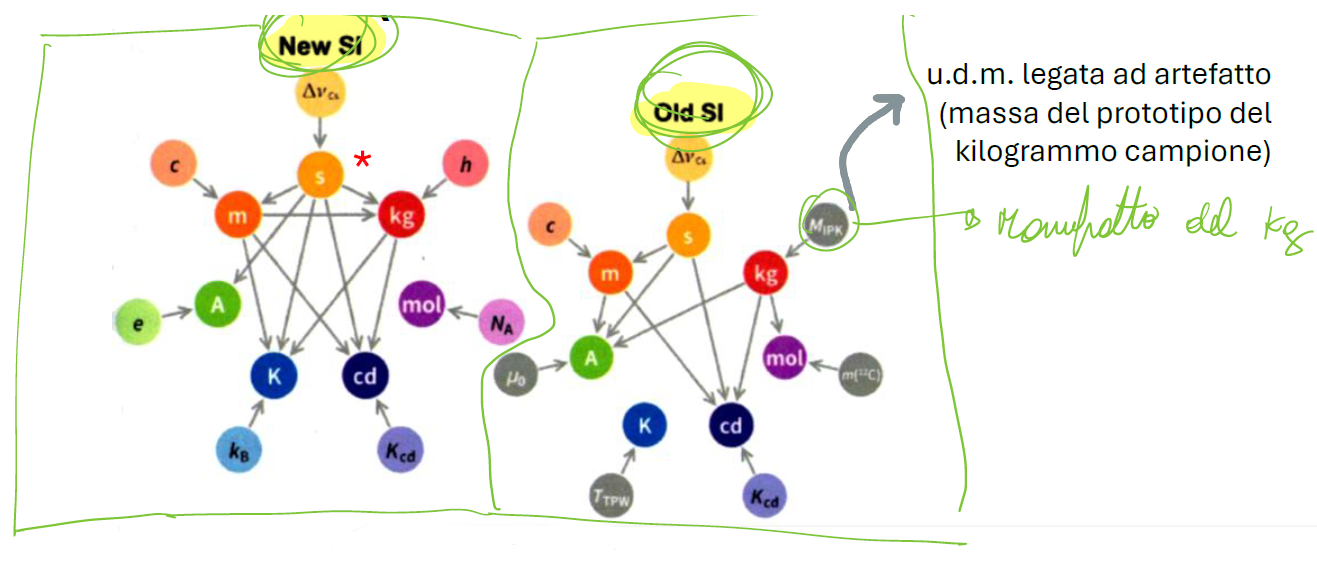
\includegraphics[scale = 0.4]{Confronto tra nuovo SI e vecchio SI.PNG}
\end{figure}

\newpage 

\section{I campioni delle unità di misura}
\footnote{Slide della prof | SDME 1.3 Metrologia - SI e Campioni | pag 25 - 41 \\  
Appunti | 2025-02-28 | pag 9 - 11 | 2025-03-04 | pag 2 - 4}

Per campioni delle unità di misura si intendono degli elementi materiali oppure fenomeni fisici utilizzati per rendere "tangibile" l'unità di misura. \newline 

Il valore del campione viene espresso mediante l'unità di misura e può non essere unitario. \newline 

Un campione deve essere: 

\begin{itemize}
    \item stabile, perché il suo valore non deve variare nel tempo 
    \item assoluto, perché il suo valore non deve dipendere dal luogo in cui è conservato 
    \item riproducibile e disseminabile, perché deve essere possibile realizzare delle copie fedeli da conservare in luoghi diversi
\end{itemize}

Per copia fedele non si intende il campione originale, ma una copia che è "poco distante" dal campione primario (l'argomento sarà approfondito di seguito). \newline 

La messa in pratica del tempo con la minor incertezza è la seguente: 

\begin{figure}[h]
    \centering
    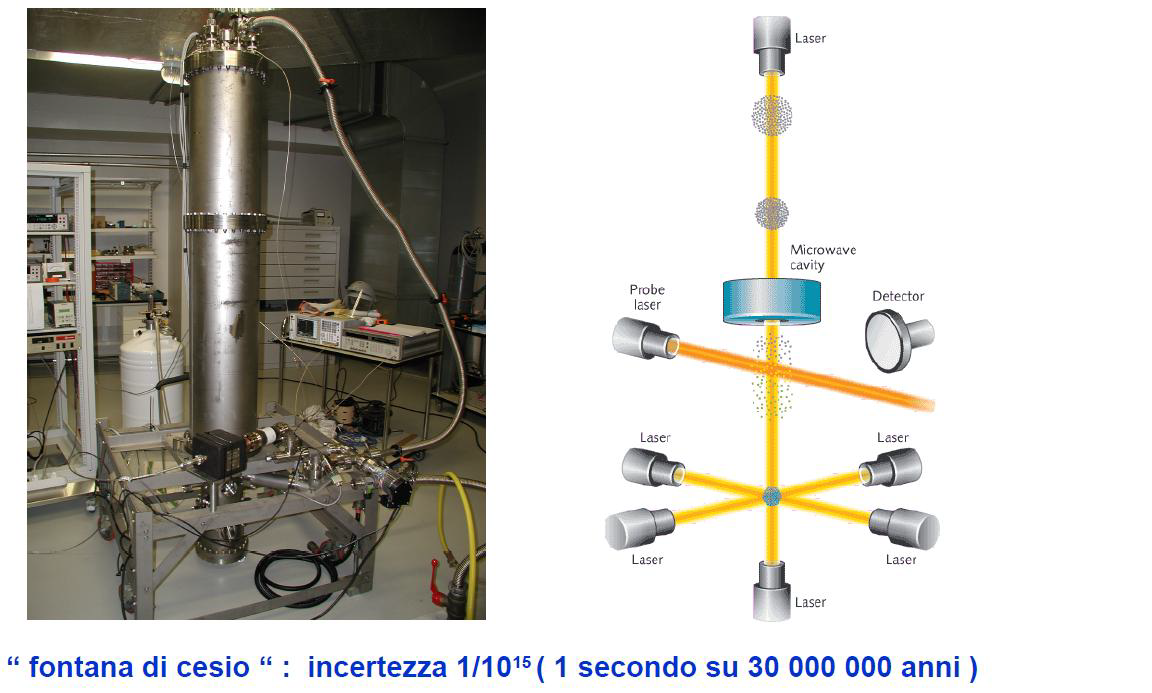
\includegraphics[scale = 0.4]{Fontana di cesio.png}
\end{figure}

cioè la fontana di cesio in cui si ha una incertezza del secondo di $10^{-15}$. \newline 

Questo processo della fontana di cesio è naturale perché ha una incertezza di 1 secondo su 30 milioni di anni. \newline 

Generalmente non è necessario conseguire incertezze così piccole, ma, siccome nella riferibilità l'incertezza aumenta, 
la realizzazione del tempo deve essere con la minor incertezza possibile. \newline 

La messa in pratica ha una sua incertezza, proprio perché è una messa in pratica. \newline 

Invece la costante assoluta non ha incertezza, per definizione. \newline 

Grazie alla riferibilità, i vari campioni fedeli sono disseminati nel mondo. \newline 

In Italia, presso l'INRiM ( Istituto Nazionale di Ricerca Metrologica) sono presenti dei campioni del tempo, che, rispetto a quello originale, hanno una incertezza maggiore. \newline 

Un esempio di campione di frequenza-tempo a Cesio 133 è l'Agilent 5071A che ha una incertezza di $10^{-12}$, 
quindi di 1 secondo su 30 000 anni, che è una incertezza maggiore rispetto al campione primario. \newline

Un altro campione molto importante è quello della lunghezza. \newline 

La messa in pratica della lunghezza è la seguente: 

\begin{figure}[h]
    \centering
    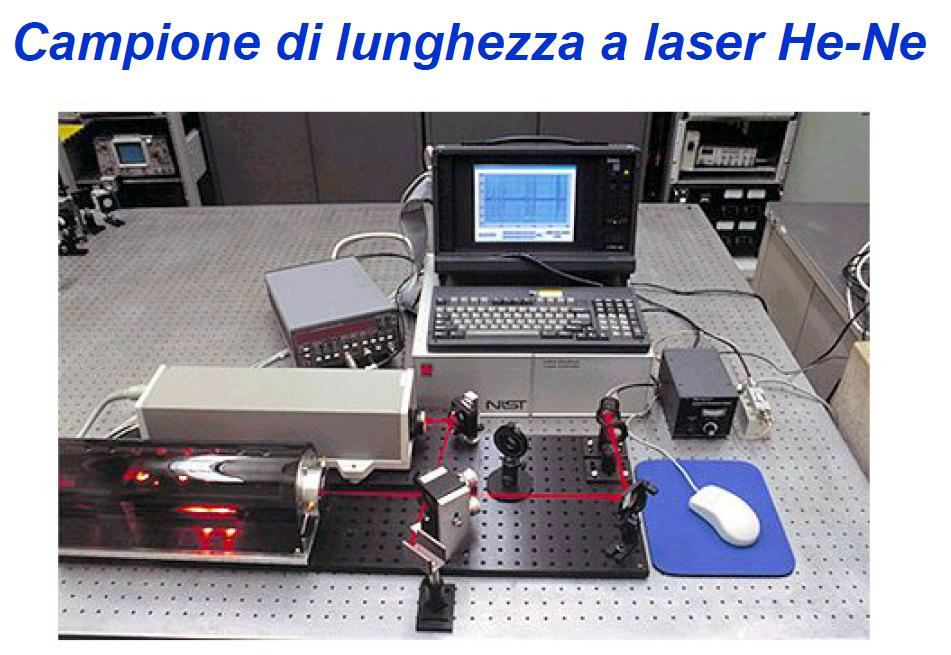
\includegraphics[scale = 0.4]{Campione della lunghezza.png}
\end{figure}


Anche questo è un campione naturale perché ha una incertezza di circa $10^{-9}$, 
cioè di 1 millimetro su 1000 km. \newline 

La realizzazione tangibile del metro, come si vede in figura, è ottenuta mediante tecniche interferometriche e presenta una incertezza 
di $\frac{4}{10^{9}}$. \newline 

Invece, per il kilogrammo, secondo il vecchio SI, si ha il prototipo internazionale di un cilindro in lega di platino-iridio conservato al BIPM: 

\begin{figure}[h]
    \centering
    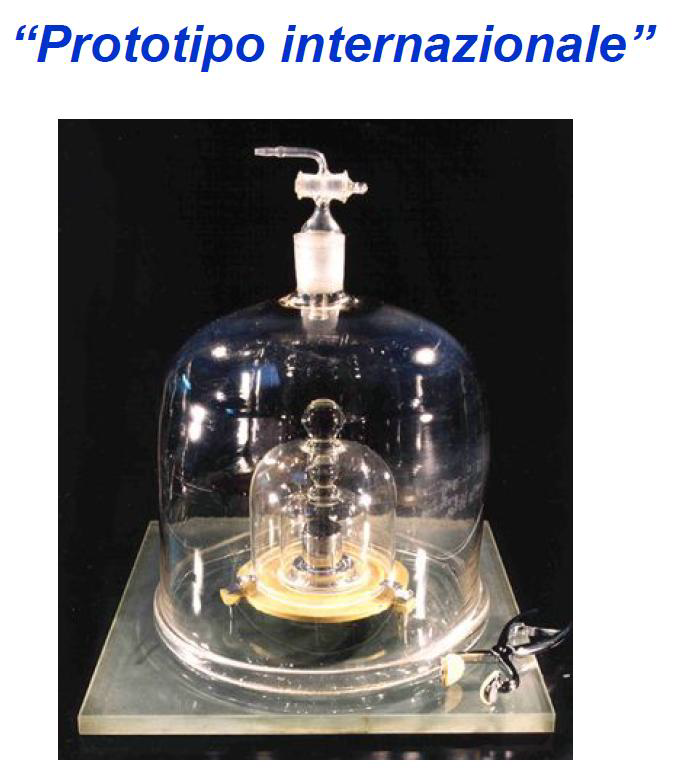
\includegraphics[scale = 0.3]{Prototipo internazionale del chilogrammo.png}
\end{figure}

Il campione di massa, rispetto a quelli precedenti, è un campione materiale. \newline 

Il ruolo degli istituiti metrologici primari è quello di realizzare e conservare i campioni primari delle diverse nazioni. \newline 

Ad esempio, in Italia è presente la copia numero 62 del prototipo internazionale, che è conservata a Torino presso l'INRiM, 
che ha una incertezza di $\frac{2}{10^{9}}$, cioè di $2\frac{ \mu g}{kg}$. \newline 

Per la u.d.m. dell'intensità di corrente, sempre secondo il vecchio SI, si ha il campione che è la bilancia elettrodinamica: 

\begin{figure}[h]
    \centering
    \includegraphics[scale = 0.3]{campione di intensità di corrente.png}
\end{figure}

\newpage 

Utilizzando la legge di Ohm, è possibile effettuare una misura indiretta della corrente. \newline 

Un altro campione di corrente è quello realizzato mediante campioni di R e di f.e.m.  con il seguente circuito: 

\begin{figure}[h]
    \centering
    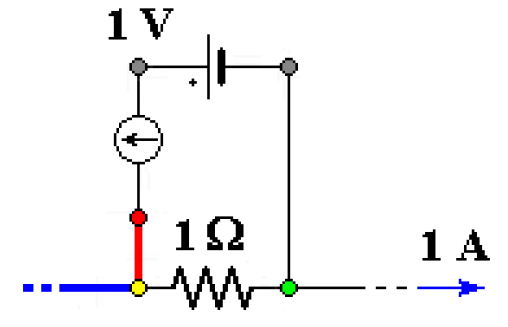
\includegraphics[scale = 0.3]{Circuito campione di corrente editato.png}
\end{figure}

Ciò è possibile grazie ai campioni primari del volt e dell'ohm, che sono presenti anche all'INRiM. \newline 

\begin{tcolorbox}
    Nelle pag 34-39 del PDF "SDME 1.3 Metrologia - SI e Campioni" è spiegato l'effetto quantistico per il campione di f.e.m. e l'effetto Josephson. \\ 
    Se vuoi approfondirlo, vai nelle slide. Sappi che il campione di f.e.m. è basato sulla misura del tempo, che è la miglior grandezza che riusciamo a misurare.   
\end{tcolorbox}

Si possono impiegare i campioni quantistici di volt e ohm per determinare una massa incognita e 
per la realizzazione pratica di un riferimento di massa. \newline 

Lo strumento è una particolare "bilancia" che confronta il watt elettrico con il watt meccanico: 
si tratta della bilancia del watt detta anche bilancia di Kibble. \newline 

Lo schema della bilancia di Kibble: 

\begin{figure}[h]
    \centering
    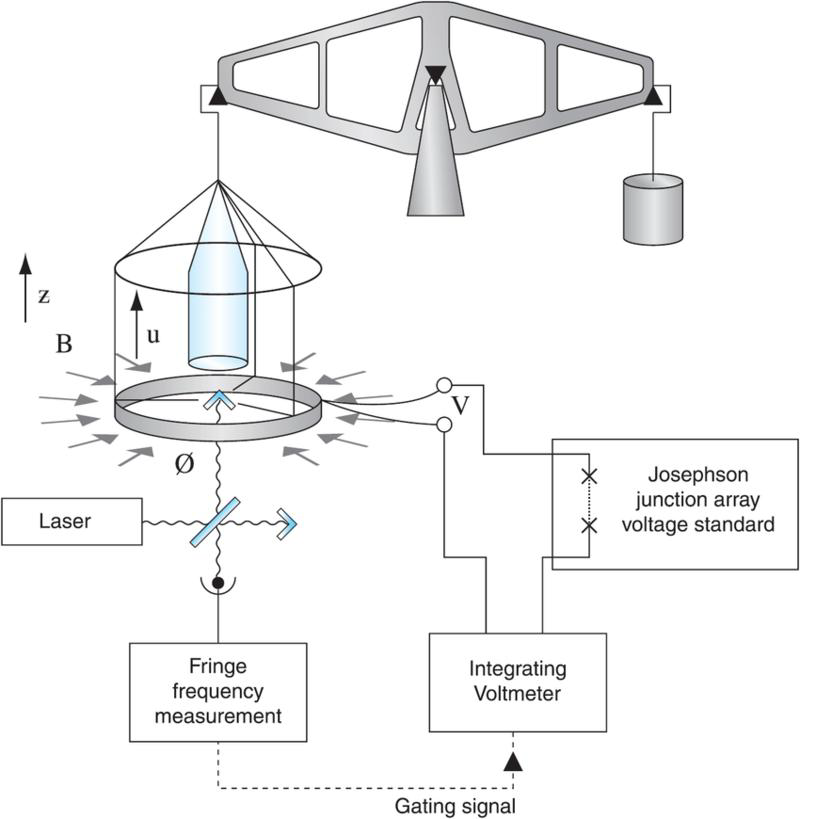
\includegraphics[scale = 0.3]{Schema della bilancia di Kibble.png}
\end{figure}


\newpage 

\section{Volt e Ohm: campioni di riferimento nazionale per l'Italia}
\footnote{Slide della prof | SDME 1.3 Metrologia - SI e Campioni | pag 42 - 44 \\  
Appunti | 2025-03-04 | pag 4 - 5}

In Italia, nel 1799, Alessandro Volta riuscì a realizzare la prima pila, 
che, ai tempi, era il generatore di f.e.m. .\newline

Invece, adesso, come campione di f.e.m. e riferimento nazionale 
viene utilizzata la pila Weston satura, che ha bisogno di essere termostata a $20 ^{\circ} C$, 
quindi la temperatura deve essere controllata. \newline 

Come campione di resistenza, viene utilizzato un cilindro in lega metallica di manganina. \newline 

\newpage 
